% Author: PokMan Ho
% Script: res.tex
% Desc: MRes thesis result section
% Input: none
% Output: none
% Arguments: 0
% Date: Jan 2020

\documentclass[../thesis.tex]{subfiles} %% use packages & commands as this main file

\begin{document}
\section{Result}
%this is the result

%% text on all result -> all graphs
\subsection{\hI} % graph stat summary
\begin{figure}[H]
    \centering
    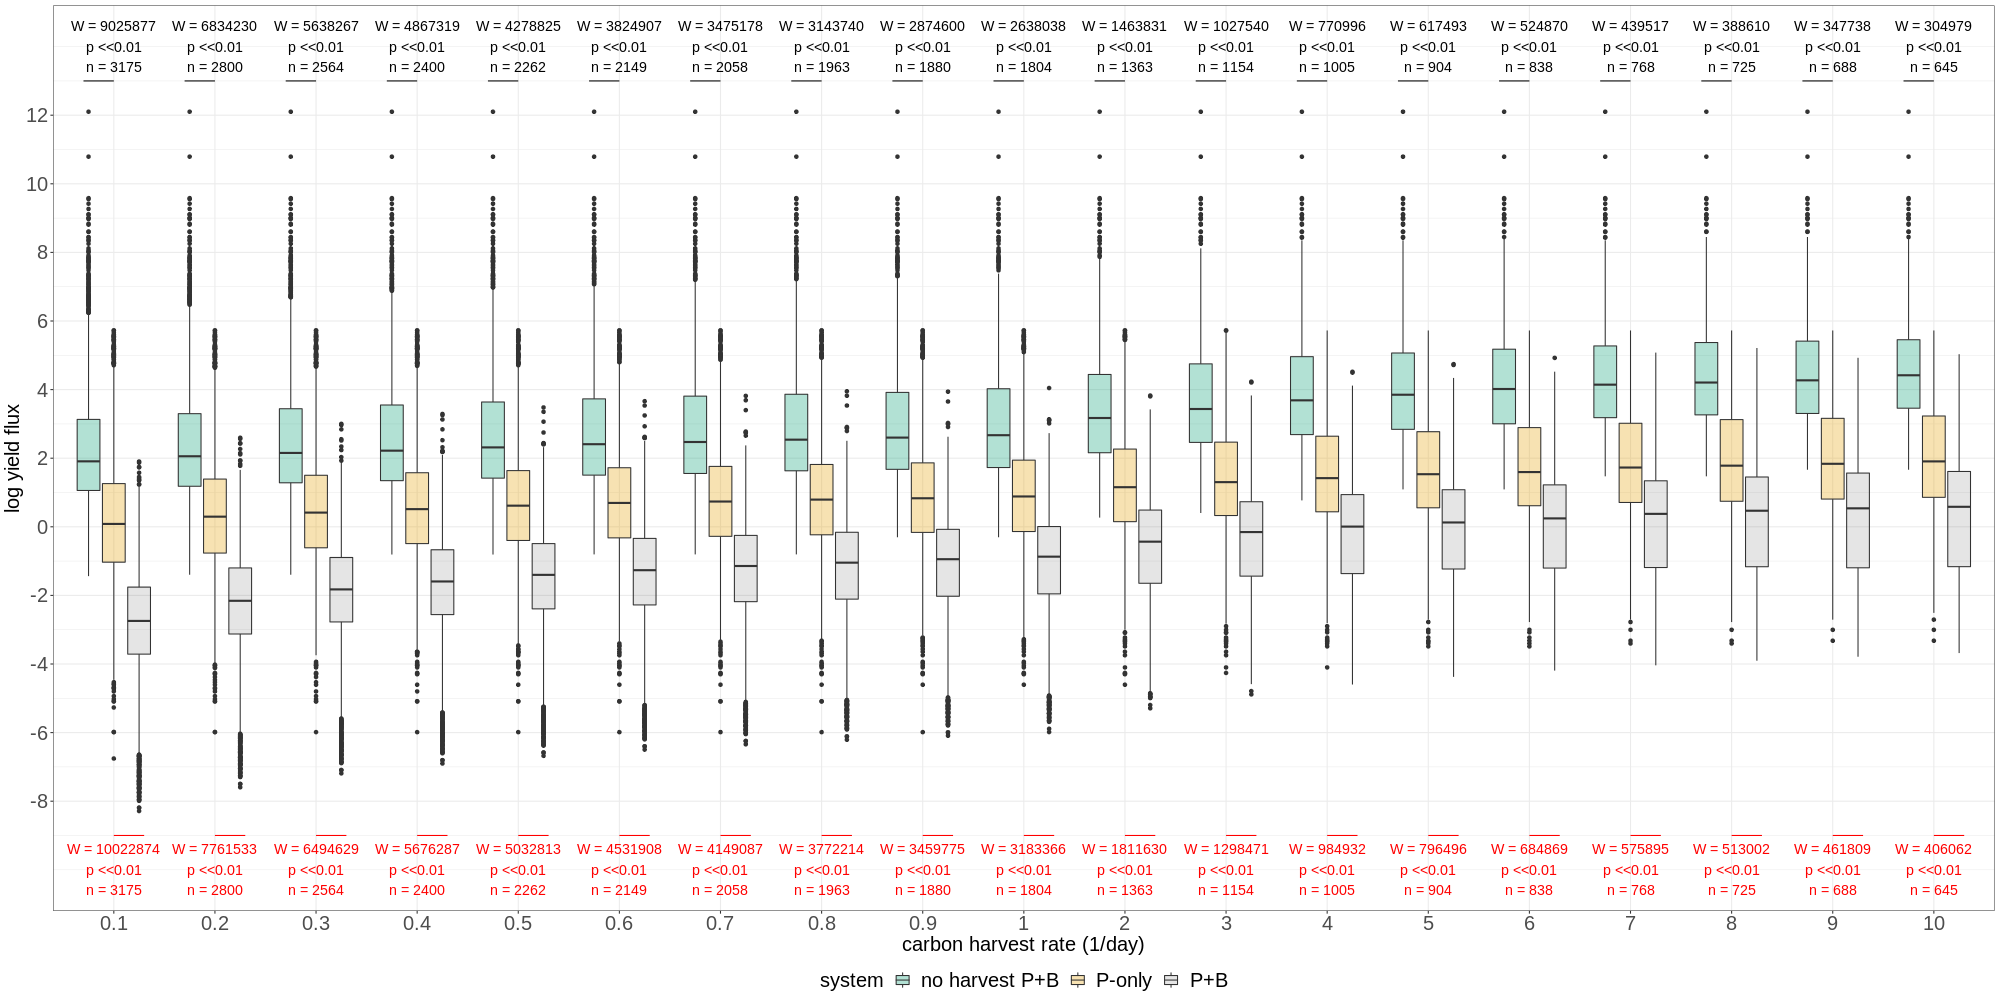
\includegraphics[width=.7\linewidth]{../result/Wilcox.png}
    \caption[Wilcox test summary]{Line graph showing Wilcox signed rank test (W-test) result (solid line) and respective p-values (dashed line) between P-only and P+B systems on ``log total carbon" and ``log yield flux" perspectives.  {\scriptsize The graph is based on the analytical simulations of the parameter hyperspace from LHS method.  Samples were divided into categories by carbon removal rate.  W-test was carried out between eqm 3 (P-only) and 4 (P+B) comparing the ranked mean distribution differences.}}
    \label{fig:wilcox}
\end{figure}

Fig.\ref{fig:wilcox} showed the W-test summary along the range of scanned removal rates ($x$).  No values were calculated for situations when $x=0$ because the organic carbon pool size was infinite for P-only systems (Table \ref{tab:eqm}).  Hence there was no valid comparisons using log values between P-only and P+B systems at $x=0$.  Generally increase in continuous removal decreased the carbon content and yield flux differences between P+B and P-only systems although the system differences remained statistical significant except when $x$ was around 0.3 to 0.4 day$^{-1}$.  At $x=0.4$ day$^{-1}$, the p-value was extremely high (p=0.79, 2dp).  The effects brought by the bacterial decomposer was not significant around that window of removal rates.


\subsection{\hII} %% text stat summary?
\begin{figure}[H]
    \centering
    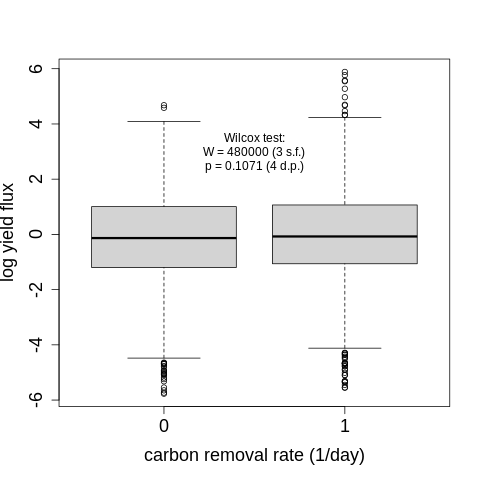
\includegraphics[width=.5\linewidth]{../result/yield.png}
    \caption[continuous harvest is not important]{Boxplot showing carbon yield distribution between no harvest ($x=0$ day$^{-1}$) and maximum harvest rate in parameter range ($x=1$ day$^{-1}$) for P+B systems.  {\scriptsize This was a comparison between the natural log values of yield flux between the minimum (0 day$^{-1}$) and maximum (1 day$^{-1}$) harvest rate carbon production.  The distributions were insignificant, although high carbon removal rate systems had the whole distribution of yields higher than that of no harvest.}}
    \label{fig:yield}
\end{figure}

[desc for yield]

\subsection{\hIII} % graph stat summary
\begin{figure}[H]
    \centering
    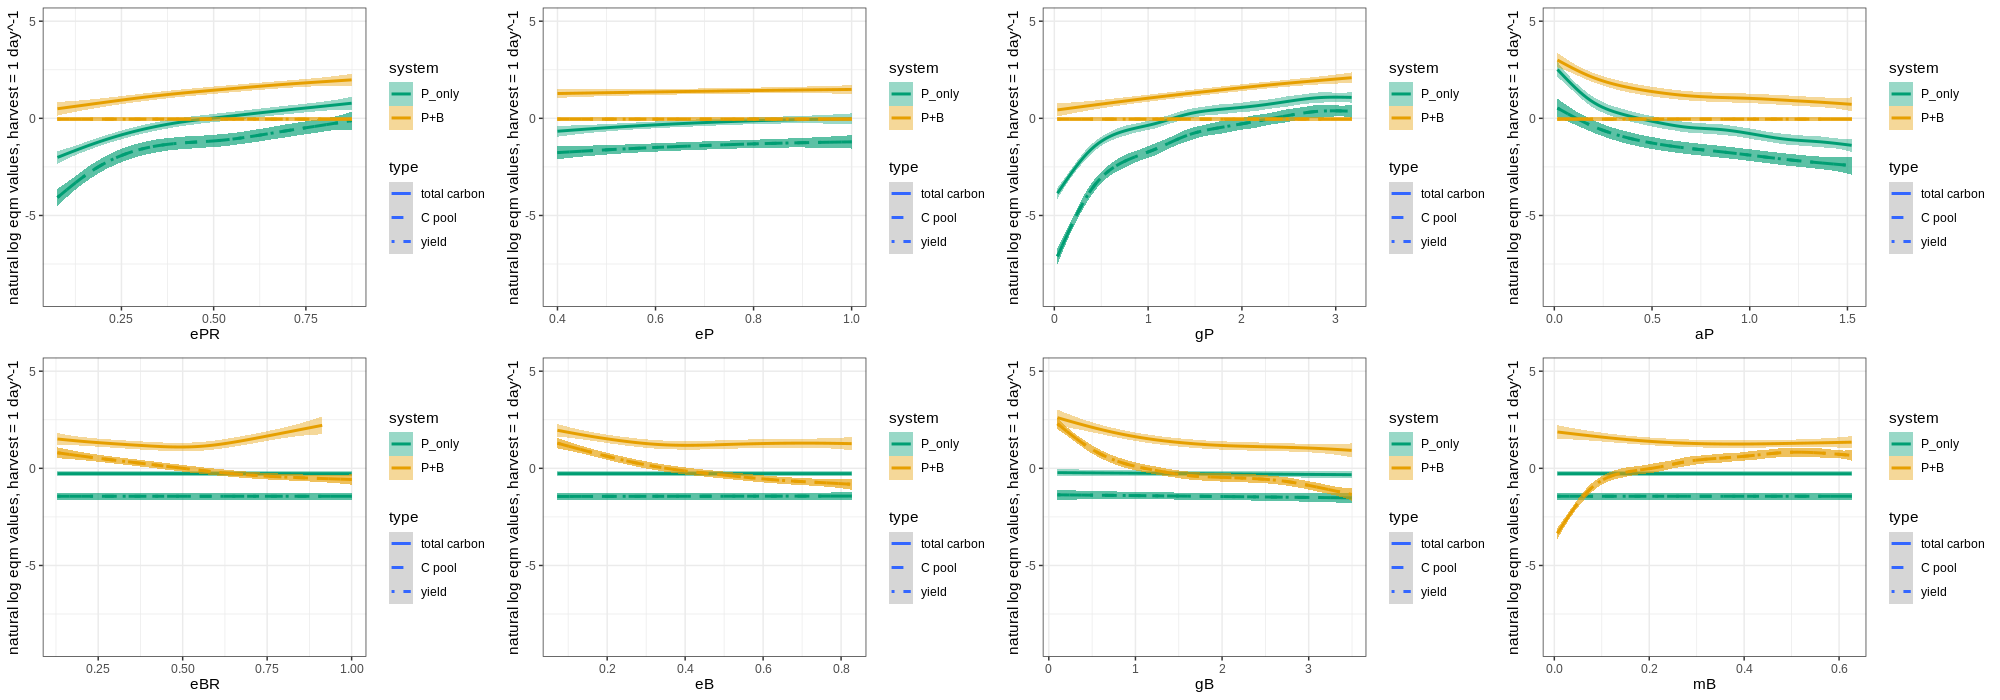
\includegraphics[width=\linewidth]{../result/var_10.png}
    \caption[95\% distribution for $x=1day^{-1}$]{Line graphs showing 95\% confidence interval for ``log total carbon" (solid line) and ``log yield flux" (dash line) based on respective parameter ranges when removal rate = 1$day^{-1}$.  {\scriptsize Simulations of $x=1$day$^{-1}$ category were summarised (n=1000) according to the eight biological parameters (Table \ref{varInTab}).  Most simulations from P+B systems had equilibrium total carbon contents significantly more (W=167624, p$\ll$0.01) than their P-only counterparts.  However for their yield flux, P+B systems were significantly less (W=346104, p$\ll$0.01) than their P-only counterparts.  The dispersion for P+B systems were also smaller than that of P-only ones.}}
    \label{fig:v10}
\end{figure}

Fig.\ref{fig:v01} was a summary of 1013 simulations under the category $x=0.1day^{-1}$.  P+B systems were significantly higher than P-only counterparts in ``total carbon" (W=416686, p$\ll$0.01) but lower in ``carbon yield flux" (W=659181, p$\ll$0.01).  The 95\% confidence intervals of P+B and P-only systems did not overlap.  In the perspective of total carbon in systems, P+B and P-only systems had the most similar result in high phytoplankton growth rates ($\gP$).  Among the parameters, only $\eBR$ had a maximum limit within the scanned parameter range.  Value of this fraction value must be smaller than 1.  For the yield flux, crossover in biological parameters were usually in the lower parameter ranges except $\mB$, which the overlap happened around the highest end of its range.  Simulations of P-only generally yielded higher than P+B systems.

Fig.\ref{fig:v10} was a summary of 1000 simulations under the category $x=1day^{-1}$.  P+B systems were significantly higher than P-only counterparts in both ``total carbon" (W=167624, p$\ll$0.01) and ``carbon yield flux"

\subsection{total carbon}
\begin{itemize}
    \item 95\% distribution don't overlap between P+B \& P-only systems
    \item highest difference happen in low $g_P$ and lowest difference in low $a_P$ regions respectively
    \item overall distribution (left histogram) has P+B distribution peaked on the right of the P-only one
    \item due to the stability in the P+B result (small 95\% interval on each solid line and across the 8 parameters), peak density of P+B higher than that of P-only
\end{itemize}

\subsection{org-C / yield}
\begin{itemize}
    \item log(yield)|$_{x=1}$ = log(org-C) + log($x$) = log(org-C)
    \item change of P parameters do not have observable effect on P+B log value (in smaller $x$ values fluctuated more)
    \item change of B parameters gave more consistent effect across parameter ranges
    \item most P+B values are higher than that of P-only
    \begin{itemize}
        \item $e_{PR}$, $g_P$, $g_B$ got (close to be) overtaken by P-only distributions
        \item $e_P$, $e_{BR}$, $e_B$ always had their distributions higher than P-only
        \item $a_P$, $m_B$ had P+B overtook P-only values at small parameter values
    \end{itemize}
    \item overall distribution (middle histogram) having P+B higher in central peak density; P-only has a wider spread in log carbon pool size
\end{itemize}

\end{document}
